\documentclass{article}
\usepackage{graphicx}
\usepackage{mathtools}
\usepackage{xfrac}
\usepackage{amsmath, amssymb}
\usepackage{listings}
\usepackage{float}
\usepackage{wrapfig}
\usepackage{tikz}
\usepackage{fullpage}
\usepackage{hyperref}
\usepackage{mathalpha}
\usepackage{tikz}
\usepackage{cite}
\usepackage{amsthm}
\usepackage{natbib}
\usepackage{multirow}
\usepackage{braket}


\newtheorem{theorem}{Proposition}[section]
\newtheorem{corollary}{Corollary}[theorem]
\newtheorem{lemma}[theorem]{Lemma}

\theoremstyle{definition}
% \newtheorem{definition}{Definition}[section]

% \theoremstyle{definition}
\newtheorem{definition}{Problem}[section]

\theoremstyle{remark}
\newtheorem*{remark}{Remark}
\newtheorem*{example}{Example}
\newtheorem*{notation}{Notation}

\title{Quantum Mechanics 1: Homework 7}
\author{David Lawton\\
        22337087}
\date{5th Nov. 2024.}

\begin{document}

\maketitle

\tableofcontents

\section{Problem 1}
A coherent state of a one-dimensional harmonic oscillator is defined to be an eigendstate of the (non-Hermitian) annihilation operator $a$
\begin{equation}
    a\ket{\lambda} = \alpha\ket{\lambda}, \quad \braket{\lambda|\lambda} = 1, \quad \alpha \in \mathbb{C}.
\end{equation}




\begin{definition}
    Find $\ket{\lambda}$.
\end{definition}
Start by recognising that since $a$ is the annihalation operator, the only non-zero eigenstate must be a infinite sum of the eigenstates $\ket{n}$ of the number operator $N = a^\dagger a$, $N\ket{n}=n\ket{n}$.
\begin{align*}
    \lambda = \sum_{n=0}^\infty c_n\ket{n}, \quad c_n \in \mathbb{C}\\
    \text{ where, } c_n = \braket{n|\lambda}
\end{align*}
We can then rewrite $\ket{\lambda}$ as
\begin{equation*}
    \ket{\lambda} = \sum_{n=0}^\infty \ket{n}\braket{n|\lambda}
\end{equation*}
but since 
\begin{equation}
    \label{eq:n state in vacuum terms}
    \ket{n}=\frac{(a^\dagger)^n}{\sqrt{n!}}\ket{0}, \bra{n}=\bra{0}\frac{a^n}{\sqrt{n!}}
\end{equation}
we can once again rewrite $\ket{\lambda}$, using Eq. \ref{eq:lambda} as well,
\begin{equation*}
    \ket{\lambda} = \sum_{n=0}^\infty \bra{0}a^n\ket{\lambda}\ket{n}=\braket{0|\lambda}\sum_{n=0}^{\infty}\frac{\alpha^n}{\sqrt{n!}}\ket{n}
\end{equation*}
Now, we simpluse the normalisation of $\ket{\lambda}$ to find $\braket{0|\lambda}=c_0$.
\begin{align*}
    1 = \braket{\lambda|\lambda} &= |c_0|^2\sum_{n=0}^\infty\frac{|\alpha|^{2n}}{n!}\\
    &= |c_0|^2e^{|\alpha|^2}\\
    ~\\
    \therefore\quad c_0&=\exp[-\frac{1}{2}|\alpha|^2]
\end{align*}
We can then write $\ket{\lambda}$ as an expansion of vectors in fock space.
\begin{equation}
    \label{eq:lambda}
    \ket{\lambda} = e^{-|\alpha|^2/2}\sum_{n=0}^\infty\frac{\alpha^n}{\sqrt{n!}}\ket{n}
\end{equation}



\begin{definition}
    Express $\ket{\lambda}$ in the form $\ket{\lambda} = f(a^\dagger)\ket{0}$.
\end{definition}
For this, we once again use Eq. \ref{eq:n state in vacuum terms} to write $\ket{\lambda}$ in terms of $a^\dagger$ operators acting on the vacuum state $\ket{0}$.
\begin{align*}
    \ket{\lambda} &= e^{-|\alpha|^2/2}\sum_{n=0}^\infty\frac{\alpha^n}{\sqrt{n!}}\frac{(a^\dagger)^n}{\sqrt{n!}}\ket{0}\\
                  &= e^{-|\alpha|^2/2}\sum_{n=0}^\infty\frac{\alpha^n}{n!}(a^\dagger)^n\ket{0}\\
\end{align*}
Therefore, using the exponential series expansion,
\begin{equation}
    \label{eq:lambda in a dagger}
    \ket{\lambda} = e^{-|\alpha|^2/2}e^{\alpha a^\dagger}\ket{0} = \exp[\alpha(a^\dagger-\frac{\alpha^*}{2})]\ket{0}
\end{equation}
which is the required form, with $f(a^\dagger) = \exp[\alpha(a^\dagger-\frac{\alpha^*}{2})]$.



\begin{definition}
    Prove the minimum uncertainty relation for this state.
\end{definition}
We must first recall that we can write the position and momentum operators in terms of annihalation and creation operators.
\begin{equation}
    X = \eta(a^\dagger+a), \quad P = \frac{i\hbar}{2\eta}(a^\dagger-a)
\end{equation}
The minimum uncertainty relation is given by
\begin{equation}
    \Delta X\Delta P \geq \frac{\hbar}{2}
\end{equation}
where $\Delta X$ and $\Delta P$ are the uncertainties in X, P respectively, defined by
\begin{equation}
    \label{eq:uncertainty}
    \Delta X = \sqrt{\braket{X^2}-\braket{X}^2}, \quad \Delta P = \sqrt{\braket{P^2}-\braket{P}^2}
\end{equation}
where the uncertainity is with respect to the state $\ket{\lambda}$. That is to say $\braket{X} = \braket{\lambda|X|\lambda}$, $\braket{X^2} = \braket{\lambda|X^2|\lambda}$ for $X$, and the same for $P$. We first calculate $\braket{X}$ and then $\braket{P}$,
\begin{align*}
    \braket{X} &= \braket{\lambda|\eta(a^\dagger+a)|\lambda}\\
               &= \eta\left(\braket{\lambda|a^\dagger|\lambda}+\braket{\lambda|a|\lambda}\right)\\
               &= \eta(\alpha^*+\alpha)\\
-------&--------------\\
    \braket{P} &= \braket{\lambda|\frac{i\hbar}{2\eta}(a^\dagger-a)|\lambda}\\
               &= \frac{i\hbar}{2\eta}\left(\braket{\lambda|a^\dagger|\lambda}-\braket{\lambda|a|\lambda}\right)\\
               &= \frac{i\hbar}{2\eta}(\alpha^*-\alpha)
\end{align*}
We then calculate $\braket{X^2}$ and $\braket{P^2}$.
\begin{align*}
    \braket{X^2} &= \braket{\lambda|\eta^2(a^\dagger+a)^2|\lambda}\\
                 &= \eta^2(\braket{\lambda|(a^\dagger)^2|\lambda}+\braket{\underset{\bra{\lambda}\alpha^*}{\underbrace{\lambda|a^\dagger}} \underset{\alpha\ket{\lambda}}{\underbrace{a|\lambda}}}+\braket{\lambda|\underset{1+a^\dagger a}{\underbrace{aa^\dagger}}|\lambda}+\braket{\lambda|a^2|\lambda})\\
                 &= \eta^2((\alpha^*)^2 + |\alpha|^2 + 1 + |\alpha|^2 + \alpha^2)\\
    -------&----------------------\\
    \braket{P^2} &= -\braket{\lambda|\frac{\hbar^2}{2\eta}(a^\dagger-a)^2|\lambda}\\
                 &= -\frac{\hbar^2}{2\eta}(\braket{\lambda|(a^\dagger)^2|\lambda}-\braket{\underset{\bra{\lambda}\alpha^*}{\underbrace{\lambda|a^\dagger}} \underset{\alpha\ket{\lambda}}{\underbrace{a|\lambda}}}-\braket{\lambda|\underset{1+a^\dagger a}{\underbrace{aa^\dagger}}|\lambda}+\braket{\lambda|a^2|\lambda})\\
                 &= -\frac{\hbar^2}{2\eta}((\alpha^*)^2 - |\alpha|^2 - 1 -|\alpha^2| +\alpha^2)
\end{align*}
Using the earlier results, we can say
\begin{equation}
    \braket{X^2} = \eta^2+\braket{X}^2, \quad \braket{P^2} = \frac{\hbar^2}{4\eta^2}+\braket{P}^2
\end{equation}
which implies, using the $\Delta X$ and $\Delta P$ definitions and Eq. \ref{eq:uncertainty},
\begin{equation*}
    \Delta X = \eta, \quad \Delta P = \frac{\hbar}{2\eta}
\end{equation*}
therefore $\Delta X\Delta P = \frac{\hbar}{2}$.

\begin{definition}
    Find the wave function $\psi_\lambda(x)$ of a coherent state in the coordinate representation.
\end{definition}
The wave function $\psi_\lambda(x)$ is defined as
\begin{equation}
    \label{eq:wave function of state lambda}
    \psi_\lambda(x) = \braket{x|\lambda}
\end{equation}
where we recall $\ket{\lambda}$ is given by Eq. \ref{eq:lambda in a dagger}. We also recall that the ground state wave function $\psi_0(x)$ is a Gaussian,
\begin{equation}
    \label{eq:psi_0}
    \psi_0(x) = \braket{x|0} = \frac{1}{\sqrt{\eta\sqrt{2\pi}}}\exp\left[-\frac{x^2}{4\eta^2}\right]
\end{equation}
We then calculate $\psi_\lambda(x)$ using Eq. \ref{eq:wave function of state lambda} and Eq. \ref{eq:lambda}.
\begin{equation*}
    \psi_\lambda(x) = \braket{x|\lambda} = e^{-|\alpha|^2/2}\sum_{n=0}^{\infty}\frac{\alpha^n}{\sqrt{n!}}\braket{x|n}
\end{equation*}
we then use two relations,
\begin{equation}
    \braket{x|n} = \psi_n(x) \text{ and } \psi_n(x) = \frac{1}{\sqrt{2^nn!}}H_n\left(\frac{x}{\eta\sqrt{2}}\right)\psi_0(x),
\end{equation}
where $H_n$ is the nth \textbf{Hermite polynomial}, to write
\begin{equation*}
    \psi_\lambda = e^{-|\alpha|^2/2}\sum_{n=0}^{\infty}\frac{\alpha^n}{n!}\frac{1}{\sqrt{2^n}}H_n\left(\frac{x}{\eta\sqrt{2}}\right)\psi_0(x)
\end{equation*}
We then write the generating function of the Hermite polynomials,
\begin{equation}
    \label{eq:generating function}
    e^{2x't-t^2} = \sum_{n=0}^{\infty}\frac{H_n(x')}{n!}t^n
\end{equation}
in our equation, $x' = \frac{x}{\eta\sqrt{2}}$ and $t = \frac{\alpha}{\sqrt{2}}$. We then have
\begin{equation*}
    \psi_\lambda(x) = \frac{1}{\sqrt{\eta\sqrt{2\pi}}}\exp\left[- \frac{x^2}{4\eta^2} + \frac{x\alpha}{\eta} - \frac{\alpha^2}{2}-\frac{|\alpha|^2}{2}\right] 
\end{equation*}
which can be shown, by completing the square, and factorising to be
\begin{equation}
    \label{eq:wave function of coherent state}
    \psi_\lambda(x) = \frac{1}{\sqrt{\eta\sqrt{2\pi}}}\exp\left[-\frac{1}{2}\left(\frac{x-2\alpha\eta}{\eta\sqrt{2}}\right)^2-\frac{\alpha}{2}\braket{P}\right]
\end{equation}

\begin{definition}
    Write $\ket{\lambda}$ as
    \begin{equation*}
        \ket{\lambda} = \sum_{n=0}^{\infty}f(n)\ket{n}
    \end{equation*}
    Show that the distribution of $|f(n)|^2$ is of the Poisson form. Find the expectation of $N$, $n$, and most probable value $n_{mp}$ of $n$, hence of $E$.
\end{definition}
Recall Eq. \ref{eq:lambda}, which is in the correct form:
\begin{equation*}
    \ket{\lambda} = e^{-|\alpha|^2/2}\sum_{n=0}^\infty\frac{\alpha^n}{\sqrt{n!}}\ket{n}
\end{equation*}
Clearly $|f(n)|^2 = |e^{-|\alpha|^2/2}\frac{\alpha^n}{\sqrt{n!}}|^2 = e^{-|\alpha|^2}\frac{|\alpha|^{2n}}{n!}$. Therefore
\begin{equation}
    \label{eq:poisson}
    |f(n)|^2 = e^{-|\alpha|^2}\frac{|\alpha|^{2n}}{n!}
\end{equation}
which is of the Poisson form ($\rho = e^-\lambda\frac{\lambda^n}{n!}$), with $\lambda = |\alpha|^2$.\\
\indent We now find the expectation value $n$ of $N$, which by substituting Eq. \ref{eq:lambda} is given by
\begin{align*}
    \braket{N} = \braket{\lambda|N|\lambda} &= \sum_{n=0}^{\infty}\braket{n|e^{-|\alpha|^2}\frac{\alpha^2n}{n!}n|n}\\
                                            &= e^{-|\alpha|^2}\sum_{n=1}^{\infty}\frac{|\alpha|^{2n}}{n!}n \quad n=1 \text{ starting value, since 0th term vanishes}\\
                                            &= |\alpha|^2e^{-|\alpha|^2}\sum_{n=1}^{\infty}\frac{|\alpha|^{2(n-1)}}{(n-1)!}
\end{align*}
Once again using the exponential series expansion, we find
\begin{equation}
    \label{eq:expectation of N}
    \braket{N} = |\alpha|^2
\end{equation}
The most probable value $n_{mp}$ of $n$ is the mode of the Poisson distribution, which is the floor of the mean. Therefore $n_{mp} \approxeq |\alpha|^2$.\\
\section{Problem 2}
Consider a particle in the potential $V(x)$,
\begin{equation}
    \label{eq:potential}
    V(x) = \begin{cases}
        -\nu\delta(x) & \text{if } x < a\\
        +\infty & \text{if } x \geq a
    \end{cases}
\end{equation}
where $\nu>0$, $a>0$.\\
\begin{definition}
    Find the wavefunctions for a scattering state. Do not normalise it.
\end{definition}
We begin by splitting the wave function into three distinct regions,
\begin{equation}
    \label{eq:wave function}
    \psi(x) = \begin{cases}
        \psi_L(x) & \text{if } x < 0\\
        \psi_M(x) & \text{if } 0 < x < a\\
        \psi_R(x) & \text{if } x > a
    \end{cases}
\end{equation}
clearly, $\psi_R(x) = 0$ since the potential is infinite, and $\psi_L(x)$, $\psi_M(x)$ are given by the Schr\"odinger equation,
\begin{equation}
    \label{eq:schrodinger}
    \frac{d^2\psi(x)}{dx^2} + k^2\psi(x) = 0, \quad k^2 = \frac{2m}{\hbar^2}E, \quad x<0
\end{equation}
since we are considering a scattering state, $E>0$. The general solution to Eq. \ref{eq:schrodinger} is
\begin{equation}
    \label{eq:general solution}
    \psi_L(x) = A_L\exp(ikx) + B_L\exp(-ikx), \quad \psi_M(x) = A_M\exp(ikx) + B_M\exp(-ikx)
\end{equation}
where $A_L$, $B_L$, $A_M$, $B_M$ are constants, which we determine using the boundary conditions. First, we use the continuity of the wave function at $x=0, a$.
\begin{align*}
    \psi_M(a) &= 0\\
    \psi_L(0) &= \psi_M(0)
\end{align*}
which gives us
\begin{align*}
    A_M\exp(ika) &= - B_M\exp(-ika) \\
    B_M &= -A_M\exp(2ika)
\end{align*}
and so, by defining $A = 2iA_M\exp(ika)$, we have
\begin{equation}
    \label{eq:psi_M}
    \psi_M(x) = A(\frac{\exp(ik(x-a))-\exp(-ik(x-a))}{2i}) = -A\sin(k(x-a))
\end{equation}
We then use the continuity of the derivative of the wave function at $x=0$.
\begin{equation*}
    A_L + B_L = A\sin(ka)
\end{equation*}
which implies
\begin{equation}
    \label{eq:psi_L}
    \psi_L(x) = 2A_Li\sin(kx) + A\sin(ka)\exp(-ikx)
\end{equation}
Then, we use integration of the Schr\"odinger equation across the discontinuity at $x=0$ to find the relation between $A_L$ and $A$.
\begin{equation}
    \label{eq:int of schrodinger}
    \frac{\hbar^2}{2m}\int_{-\epsilon}^{\epsilon}\frac{d^2\psi(x)}{dx^2}dx + \int_{-\epsilon}^{\epsilon}\nu\delta(x)\psi(x)dx = -E\int_{-\epsilon}^{\epsilon}\psi(x)dx
\end{equation}
Then let $\epsilon\to0$ to find
\begin{equation*}
\frac{d\psi}{dx}\Big|_{0^-}^{0^+} + \frac{2m\nu}{\hbar^2}\psi(0) = 0
\end{equation*}
since the last term vanishes as $\psi(x)$ is continuous at $x=0$. We then fill in $\psi_L'(0)$ and $\psi_M'(0)$ to find
\begin{align*}
    \psi_M'(0) - \psi_L'(0) &= \frac{2m\nu}{\hbar^2}\psi_M(0)\\
    kA\cos(ka) + 2iA_Lk - iAk\sin(ka) &= \frac{2m\nu}{\hbar^2}(A\sin(ka))\\
    \Rightarrow A_L &= \frac{A}{2ik}\left(\frac{2m\nu}{\hbar^2}\sin(ka) + ik\sin(ka) - k\cos(ka)\right)
\end{align*}
$\psi_L(x)$ can then be written as
\begin{align*}
    \psi_L(x) &= \frac{A}{k}\left(\frac{2m\nu}{\hbar^2}\sin(ka) + ik\sin(ka) - k\cos(ka)\right)\sin(kx) + A\sin(ka)(\cos(kx)-i\sin(kx))\\
              &= \frac{A}{k}\left(\frac{2m\nu}{\hbar^2}\sin(ka)\sin(kx) + ik\sin(ka)\sin(kx) - k\cos(ka)\sin(kx) - iAk\sin(ka)\sin(kx) + iA\sin(ka)\cos(kx)\right)\\
              &= A\left[\frac{2m\nu}{\hbar^2}\sin(ka)\sin(kx) +\sin(ka)\cos(kx) - k\cos(ka)\sin(kx)\right] + A\sin(ka)\\
              &= A\frac{2m\nu}{\hbar^2}\sin(ka)\sin(kx) - A\sin(k(x-a))
\end{align*}
Therefore, the wave function for a scattering state of a potential described by Eq. \ref{eq:potential} is
\begin{equation}
    \label{eq:wave function of scattering state}
    \psi(x) = \begin{cases}
        A\frac{2m\nu}{\hbar^2}\sin(ka)\sin(kx) - A\sin(k(x-a)) & \text{if } x < a\\
        -A\sin(k(x-a)) & \text{if } 0 < x < a\\
        0 & \text{if } x > a
    \end{cases}
\end{equation}
\begin{definition}
    Find wave function for bound states, and a quantisation condition for the bound state spectrum. Do not normalise it.
\end{definition}
Once again we split the wave function into three distinct regions,
\begin{equation}
    \label{eq:wave function bound}
    \psi(x) = \begin{cases}
        \psi_L(x) & \text{if } x < 0\\
        \psi_M(x) & \text{if } 0 < x < a\\
        \psi_R(x) = 0 & \text{if } x > a
    \end{cases}
\end{equation}
and states for which $E<0$ are bound states. We can also write $E' = -E$ for simplicity. The Schr\"odinger equation is then solved by the general solution
\begin{equation}
    \label{eq:general solution bound}
    \psi(x) = Ae^{\kappa x} + Be^{-\kappa x}, \quad \kappa^2 = \frac{2m}{\hbar^2}E'
\end{equation}
We then annalyse the behaviour at the limits of each region, and the continuity of the wave function at $x=0, a$.
\begin{equation*}
    \psi_L(-\infty) = 0 \quad\Rightarrow B_L = 0
\end{equation*}
\begin{align*}
    \psi_M(a) &= 0\\
    \psi_L(0) &= \psi_M(0)
\end{align*}
which gives us
\begin{align*}
    A_M\exp(\kappa a) &= - B_M\exp(-\kappa a)\\
    \Rightarrow \psi_M(x) &= C(\exp(\kappa(x-a))-\exp(-\kappa(x-a))),\quad C = A_Me^{\kappa a}\\
    &= D\sinh(\kappa(x-a))
\end{align*}
using the first condition, and then
\begin{equation*}
    A = -De^{-\kappa x}\sinh(\kappa a)
\end{equation*}
using the second condition. To find the quantisation condition, we integrate the Schr\"odinger equation across the discontinuity at $x=0$, as in Eq. \ref{eq:int of schrodinger}.
\begin{align*}
    \psi_M'(0) - \psi_L'(0) &= -\frac{2m\nu}{\hbar^2}\psi(0)\\
    \kappa D \cosh(\kappa a) + \kappa D \sinh(\kappa a) &= \frac{2m\nu}{\hbar^2}D\sinh(\kappa a)\\
    \Rightarrow \kappa e^{\kappa a} &= \frac{m\nu}{\hbar^2}(e^{\kappa a} - e^{-\kappa a})\\
    \frac{\kappa}{1-e^{-2\kappa a}} &= \frac{m\nu}{\hbar^2}\\
    \Rightarrow e^{2\kappa a} \left(1 - \frac{\kappa\hbar^2}{m\nu}\right) &= 1
\end{align*}
This leads us to the quantisation condition,
\begin{equation}
    \label{eq:quantisation condition}
    e^{2\kappa a} = \frac{m\nu}{m\nu - \hbar\sqrt{2mE'}}
\end{equation}
\begin{definition}
    Show that the energy quantisation condition can be written in the form
    \begin{equation}
        \label{eq:quantisation condition form}
        \frac{z}{W} = 1 - e^{-z}
    \end{equation}
    where $z$, $W$ are yet to be determined.\\
    Sketch plots of the left and right hand sides of the energy quantisation condition for $W=1/2, 2$.
    Prove that there exist at most only one bound state that is the ground state of the system, find values of $W$ for which there is a ground state.
\end{definition}
the quantisation condition Eq. \ref{eq:quantisation condition} can be easily manipulated to the required form by defining $z = 2\kappa a$ and $W = \frac{2m\nu a}{\hbar^2}$, and doing some simple algebra as below,
\begin{align*}
    \frac{\kappa}{1-e^{-z}} &= \frac{m\nu}{\hbar^2}\\
    \Rightarrow \quad \frac{\kappa \hbar^2}{m\nu} &= 1 - e^{-z}\\
    \Rightarrow \quad \frac{z\hbar^2}{2am\nu} &= 1 - e^{-z}\\
    \Rightarrow \quad \frac{z}{W} & = 1-e^{-z}
\end{align*}
thusly illustrating Eq. \ref{eq:quantisation condition form}.\\
\indent We then sketch the left and right hand sides of the energy quantisation condition for $W=1/2, 2$, in figure \ref{fig: quantisation}.\\
\begin{figure}[H]
    \centering
    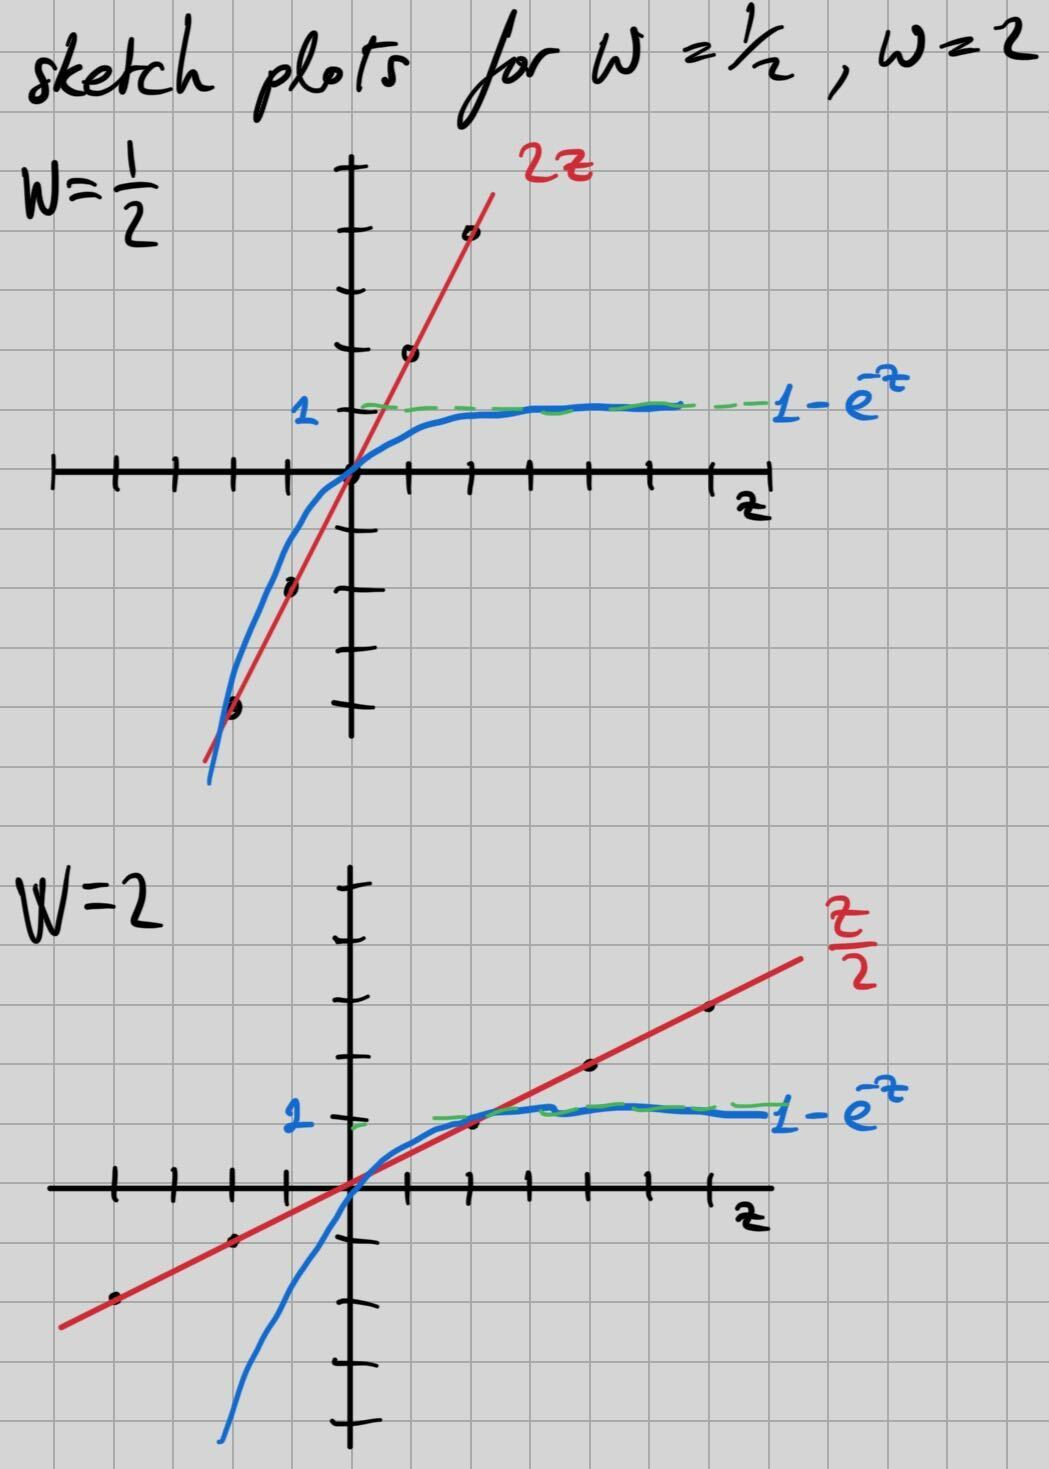
\includegraphics[width=0.5\textwidth]{quantisation_condition_plot.jpg}
    \caption{\label{fig: quantisation}Plot of the left and right hand sides of the energy quantisation condition for $W=1/2, 2$. Note that for $W=1/2$, there are no solutions as there are no non zero intersections of the two curves for $z>0$. Conversely, for $W=2$, there is one solution.}
\end{figure}
Since both sides of the equation pass through the origin, and the right hand side has a constantly decreasing derivative, it is clear that there are solutions only for $W$ such that 
\begin{equation*}
    \frac{1}{W} = \frac{d}{dz}\left(\frac{z}{W}\right) < \left[\frac{d}{dz}\left(1-e^{-z}\right)\right]_{z=0} = 1
\end{equation*}
this implies that there exists a bound state only for $W>1$. It is also implied, since linear and exponential functions can only intersect twice, that there is only one state, as one intersection is always at the origin.\\
\begin{definition}
    Find the ground state energy $E_0$ in the limit $W\rightarrow\infty$. Explain the result obtained.
\end{definition}
for $W\rightarrow\infty$, clearly there are only two possible $z$-values. The first is $z=0$, which is not a solution, since only $z>0$ values are relevant. The second is $z=W\rightarrow\infty$, which is a solution, as
\begin{equation*}
    1 = \lim_{W\rightarrow\infty}\frac{W}{W} = 1 - e^{-z} = 1 - e^{-W} = 1
\end{equation*}
The result obtained implies
\begin{equation*}
    \sqrt{{\frac{2mE'}{\hbar^2}}} = \kappa = \frac{m\nu}{\hbar^2}
\end{equation*}
which then leads to the conclusion,
\begin{equation}
    \label{eq:ground state energy}
    E = -E' = \frac{m\nu^2}{2\hbar^2}
\end{equation} 
this goes to infinity if $W\rightarrow\infty$ because of $\nu\rightarrow\infty$ (infinitely deep delta function), but if $a\rightarrow\infty$ (no wall), the energy $E = E'$ depends only on the strength of the delta function.\\
\end{document}